\section{方差控制}
\label{sec:sgd-variance}

上一节的误差界都有一项与噪声方差$\sigma^2$成正比。目标和精度要求固定时，把这一项压下去就能用更少的更新达到相同的结果。有哪些办法减小读数的方差，每种办法又要付出多少读取、存储和维护成本？这两件事必须一起看，方差减小不等于总计算减少。

三类办法依次是：一次多读几项，改变抽项的分布，利用已经读过的梯度。

\subsection{小批量与梯度累积}
\label{sec:sgd-minibatch}

\paragraph{批量平均的方差}
最直接的办法是一次读$B$项取平均。设给定历史后$\hat{\bm{g}}_1,\ldots,\hat{\bm{g}}_B$独立同分布，且都是$\nabla f(\bm{x})$的无偏读数，条件方差为$\sigma^2$。\term{小批量}（mini-batch）读数是
\begin{equation}
 \hat{\bm{g}}_{(B)}=\frac{1}{B}\sum_{k=1}^{B}\hat{\bm{g}}_k.
 \label{eq:sgd-minibatch}
\end{equation}

记$\bm{\zeta}_k=\hat{\bm{g}}_k-\nabla f(\bm{x})$。把平方展开，分成平方项和交叉项：
\[
 \mathbb{E}\Bigl[\Bigl\lVert\frac{1}{B}\sum_{k}\bm{\zeta}_k\Bigr\rVert_2^2\;\Big|\;\mathcal{F}^{(t)}\Bigr]
 =\frac{1}{B^2}\sum_{k}\mathbb{E}[\lVert\bm{\zeta}_k\rVert_2^2\mid\mathcal{F}^{(t)}]+\frac{1}{B^2}\sum_{k\neq l}\mathbb{E}[\langle\bm{\zeta}_k,\bm{\zeta}_l\rangle\mid\mathcal{F}^{(t)}].
\]

给定历史时$\bm{\zeta}_k$和$\bm{\zeta}_l$独立且条件均值为零，所以内积的条件期望等于两个条件均值的内积，即零。平方项一共$B$个，所以
\begin{equation}
 \operatorname{Var}\bigl[\hat{\bm{g}}_{(B)}\mid\mathcal{F}^{(t)}\bigr]=\frac{\sigma^2}{B}.
 \label{eq:sgd-minibatch-variance}
\end{equation}
关键在于交叉项消失，这是独立带来的。若读数之间相关，交叉项不再为零，须把它们的协方差保留在展开式中。

\paragraph{无放回的方差}
从$N$项中无放回地抽$B$项，读数不独立，交叉项有确定的值。记$\bm{v}_i=\nabla f_i(\bm{x})-\nabla f(\bm{x})$，它们的和是零，平均平方是$\sigma^2$。对$\lVert\sum_i\bm{v}_i\rVert_2^2=0$展开，得到
\[
 \sum_{i}\lVert\bm{v}_i\rVert_2^2+\sum_{i\neq j}\langle\bm{v}_i,\bm{v}_j\rangle=0.
\]
所以不同的两项的内积平均是$-\sigma^2/(N-1)$。

把这个值代入上面的展开式，交叉项一共$B(B-1)$个，得到
\begin{equation}
 \operatorname{Var}\bigl[\hat{\bm{g}}_{(B)}\mid\mathcal{F}^{(t)}\bigr]=\frac{\sigma^2}{B}\cdot\frac{N-B}{N-1}.
 \label{eq:sgd-minibatch-no-replacement}
\end{equation}
因子$(N-B)/(N-1)$小于$1$。$B=N$时方差为零，正是读完全部的情形。

在三项目标的$x^\star$处核对，这时$\sigma^2=56/3$，读数$(4,2,-6)$的和是零。取$B=2$无放回，三种配对的平均读数是$3,\,-1,\,-2$，平方的平均是
\[
 \frac{9+1+4}{3}=\frac{14}{3}.
\]
公式~\eqref{eq:sgd-minibatch-no-replacement}给出同一结果：$\tfrac{56/3}{2}\cdot\tfrac12=\tfrac{14}{3}$。有放回的$B=2$则是$28/3$，多了一倍。

\begin{BookInlineFigure}
  \centering
  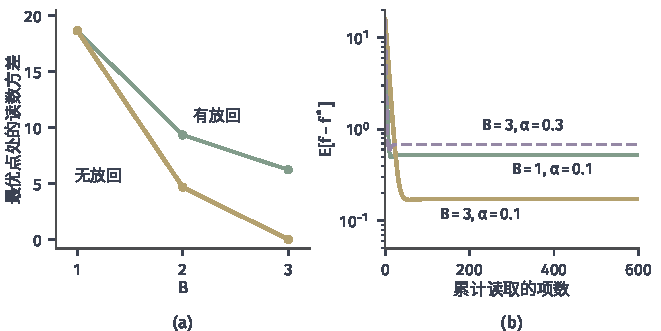
\includegraphics[width=112mm]{figures/05-optimization/05-stochastic-optimization/matplotlib/sgd-minibatch-variance/figure.pdf}
  \caption{小批量的方差与成本，三项目标。(a)最优点处读数方差随批量的变化，绿线有放回，黄线无放回，$B=3$时无放回的方差为零。(b)从$x^{(0)}=5$出发的期望目标差，由精确递推算出，横轴是累计读取的项数。绿线$B=1$，黄线$B=3$且步长相同，紫色虚线$B=3$且步长乘以$3$。}
  \label{fig:sgd-minibatch-variance}
\end{BookInlineFigure}

\paragraph{方差减小不等于计算减少}
式~\eqref{eq:sgd-minibatch-variance}让噪声项除以$B$，但读取量乘以$B$。图~\ref{fig:sgd-minibatch-variance}(b)说明了两者的权衡。步长不变时，$B=3$的噪声底从$0.53$降到$0.17$；把步长也放大$3$倍，保持每次读取走过的距离不变，$B=3$的噪声底是$0.68$，并不比$B=1$更好，初始阶段的下降也差不多。在步长可以随批量调整的范围内，增加批量和缩小步长的效果大体相同，总读取量并没有节省。

增加批量的价值在别处：多个读数可以并行计算，矩阵运算可以成批进行，方差小了也允许使用更稳健的步长。这些是实现上的收益，须按实际硬件单独计算。

\paragraph{梯度累积}
批量太大、一次放不进内存时，可以把它拆成若干微批量，分别算梯度后加起来，只更新一次，这称为\term{梯度累积}（gradient accumulation）。设批量$B$拆成微批量，大小为$n_1,\ldots,n_K$，$\sum_kn_k=B$。设第$k$个微批量的平均读数为$\hat{\bm{g}}_k$，累积时必须按样本数加权：
\begin{equation}
 \hat{\bm{g}}_{(B)}=\sum_{k=1}^{K}\frac{n_k}{B}\hat{\bm{g}}_k.
 \label{eq:sgd-accumulation}
\end{equation}

\begin{BookInlineFigure}
  \centering
  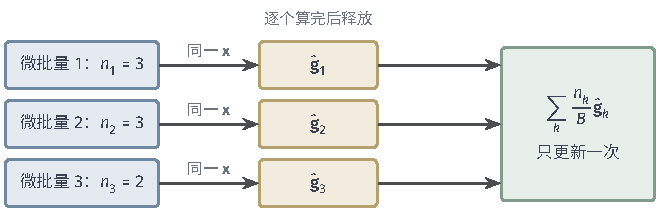
\includegraphics[width=112mm]{figures/05-optimization/05-stochastic-optimization/tikz/sgd-gradient-accumulation/figure.pdf}
  \caption{梯度累积。批量$8$拆成大小为$3,3,2$的微批量。参数在整个过程中保持不变，每个微批量的梯度算完就可以释放它占用的样本与中间结果。累积时按$n_k/B$加权，全部读完后才更新一次。}
  \label{fig:sgd-gradient-accumulation}
\end{BookInlineFigure}

图~\ref{fig:sgd-gradient-accumulation}显示了三个要求。第一，整个累积过程中参数$\bm{x}$不变，否则各微批量的梯度算在不同的点上，加起来不是一个点的梯度。第二，目标函数不变，包括确定的正则项只加一次。第三，权重按样本数计。三项目标上把第一、二项作为一个微批量，第三项单独作为一个，$x=2$处
\[
 \frac23\cdot\frac{5+4}{2}+\frac13\cdot(-3)=2,
\]
与三项的平均相同。若不加权，直接平均两个微批量的读数，得到$(4.5-3)/2=0.75$，答案错了。

读数若还依赖批内统计量，例如用批内均值做归一化，拆开后微批量的统计量与整批不同，累积结果不再等于整批的结果，这些统计量要在整批范围内统一更新。

梯度累积减少的只是同时占用的存储，总读取量仍是$B$。它不是一种降低方差的新办法，只是用更长的时间换更少的内存，方差与整批相同。

\subsection{非均匀抽样}
\label{sec:sgd-importance}

有些项的梯度大，有些小。均匀抽样对所有项一视同仁，把更多机会给“重要”的项，能否减小方差？

\paragraph{逆概率权重}
以固定的正概率$p_1,\ldots,p_N$抽项，$\sum_ip_i=1$。为使条件均值仍是完整梯度，要给读数加上逆概率权重：
\begin{equation}
 \hat{\bm{g}}=\frac{1}{Np_i}\nabla f_i(\bm{x})+\nabla r(\bm{x}).
 \label{eq:sgd-importance-estimator}
\end{equation}
确定的正则梯度$\nabla r$无需抽样，单独加入。条件均值按概率加权直接计算，分母上的$p_i$与概率相消：
\[
 \sum_{i=1}^{N}p_i\cdot\frac{1}{Np_i}\nabla f_i(\bm{x})+\nabla r(\bm{x})=\frac{1}{N}\sum_{i=1}^{N}\nabla f_i(\bm{x})+\nabla r(\bm{x}).
\]
这就是式~\eqref{eq:sgd-finite-sum-regularized}的完整梯度。这种做法称为\term{非均匀抽样}（non-uniform sampling），权重也称重要性权重。

权重不能省略。第~\ref{sec:sgd-unbiased}小节的概率$(1/2,1/4,1/4)$在不加权时，实际被最小化的是加权目标$\tfrac12f_1+\tfrac14f_2+\tfrac14f_3$，它的梯度是
\[
 \frac12(x+3)+\frac14\cdot2x+\frac14(3x-9)=\frac74x-\frac34.
\]
零点是$x=3/7$，而不是$x^\star=1$。算法的不动点取决于读数的条件均值，而不取决于更新的形式。

\paragraph{不同概率下的二阶矩}
无偏之后比较方差，只需比较二阶矩，因为均值已固定。设$r=0$，读数$\tfrac{1}{Np_i}\nabla f_i$的二阶矩是
\begin{equation}
 M(\bm{p})=\sum_{i=1}^{N}p_i\Bigl\lVert\frac{\nabla f_i(\bm{x})}{Np_i}\Bigr\rVert_2^2=\frac{1}{N^2}\sum_{i=1}^{N}\frac{\lVert\nabla f_i(\bm{x})\rVert_2^2}{p_i}.
 \label{eq:sgd-importance-second-moment}
\end{equation}

由Cauchy--Schwarz不等式，
\[
 \Bigl(\sum_i\lVert\nabla f_i\rVert_2\Bigr)^2\leq\Bigl(\sum_i\frac{\lVert\nabla f_i\rVert_2^2}{p_i}\Bigr)\Bigl(\sum_ip_i\Bigr).
\]
于是$M(\bm{p})$的最小值是$(\sum_i\lVert\nabla f_i\rVert_2)^2/N^2$，在$p_i\propto\lVert\nabla f_i(\bm{x})\rVert_2$时取到。最优概率依赖当前点，而算出它需要读完全部的项，这与抽样的目的相矛盾。

在三项目标的$x^\star$处，读数是$(4,2,-6)$，代入式~\eqref{eq:sgd-importance-second-moment}比较三种概率：
\[
 \begin{aligned}
 \bm{p}=\bigl(\tfrac13,\tfrac13,\tfrac13\bigr):\quad&M=\tfrac{56}{3}\approx18.67,\\
 \bm{p}\propto(L_1,L_2,L_3)=\bigl(\tfrac16,\tfrac13,\tfrac12\bigr):\quad&M=20,\\
 \bm{p}\propto(\lvert4\rvert,\lvert2\rvert,\lvert{-6}\rvert)=\bigl(\tfrac13,\tfrac16,\tfrac12\bigr):\quad&M=16.
 \end{aligned}
\]
常用的$p_i\propto L_i$在这个点上比均匀更差。这种选择有另外的好处：加权后各项的光滑常数$L_i/(Np_i)$相同，都等于$\bar{L}=\tfrac1N\sum_iL_i=2$，而不再是$L_{\max}=3$。依赖逐项光滑常数的步长上界因此放宽。

\begin{BookInlineFigure}
  \centering
  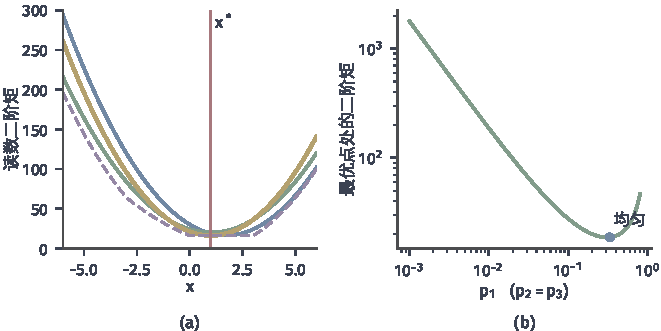
\includegraphics[width=112mm]{figures/05-optimization/05-stochastic-optimization/matplotlib/sgd-importance-sampling/figure.pdf}
  \caption{非均匀抽样的二阶矩，三项目标。(a)不同固定概率下的读数二阶矩随$x$的变化：蓝线均匀，绿线$p_i\propto L_i$，黄线$p_i\propto\lvert f_i'(x^\star)\rvert$，紫色虚线是每点都用最优概率的下包络，红线是$x^\star$。(b)最优点处二阶矩随$p_1$的变化，$p_2=p_3=(1-p_1)/2$，两轴取对数，蓝点是均匀抽样。}
  \label{fig:sgd-importance-sampling}
\end{BookInlineFigure}

图~\ref{fig:sgd-importance-sampling}(a)显示，三条曲线在不同位置各有胜负。没有哪个固定的分布处处最好，这是最优概率依赖$\bm{x}$的直接表现。图(b)说明另一个危险：概率过小会放大读数。$p_1=0.01$时第一项读数被放大$1/(3\cdot0.01)\approx33$倍，$x^\star$处的二阶矩升到约$187$，是均匀抽样的十倍。一项只要可能有非零梯度，就要给它不太小的概率。

代价方面要算三笔账。计算概率需要各项的$L_i$或梯度范数的估计；维护离散分布、每次抽样需要合适的数据结构，概率更新后还要维护；若各项尺度相近，这些投入得不到回报。只有各项差异明显、概率容易得到时，非均匀抽样才值得使用。

\subsection{SVRG}
\label{sec:sgd-svrg}

小批量靠多读减小方差，方差只能按$1/B$下降，到最优点也不消失。有没有办法让读数的方差随迭代点靠近解而自动趋于零？图~\ref{fig:sgd-term-gradients}(b)的观察给出了线索：三条单项导数虽然不同，但都是光滑变化的，在相邻两点的差别不大。

\paragraph{主要思想}
控制变量的想法是：如果要估计一个数，手里还有一个与它高度相关且均值已知的量，就可以用它来纠偏。这里的已知量是一个旧点的梯度。

选一个快照点$\tilde{\bm{x}}$，事先计算好它的完整梯度$\nabla f(\tilde{\bm{x}})$。此后每一步抽$i$，用同一项在当前点和快照点的梯度差，加上快照的完整梯度：
\begin{equation}
 \hat{\bm{g}}=\nabla f_i(\bm{x})-\nabla f_i(\tilde{\bm{x}})+\nabla f(\tilde{\bm{x}}).
 \label{eq:sgd-svrg-direction}
\end{equation}
这就是\term{SVRG}（stochastic variance reduced gradient）\scite{johnson2013accelerating}的方向。$\nabla f_i(\tilde{\bm{x}})$称为\term{控制变量}（control variate）。

对$i$求条件平均，第一项是$\nabla f(\bm{x})$，后两项相消：
\[
 \mathbb{E}[\hat{\bm{g}}\mid\mathcal{F}^{(t)}]=\nabla f(\bm{x})-\nabla f(\tilde{\bm{x}})+\nabla f(\tilde{\bm{x}})=\nabla f(\bm{x}).
\]
所以$\hat{\bm{g}}$条件无偏，这里不需要任何关于$\tilde{\bm{x}}$的假设。方差却取决于$\bm{x}$和$\tilde{\bm{x}}$的距离：若$\bm{x}=\tilde{\bm{x}}$，$\hat{\bm{g}}$恰为完整梯度，一点噪声也没有。

三项目标的读数是一次函数，修正后的方向很简单：
\[
 \hat{g}=a_i(x-\tilde{x})+f'(\tilde{x}).
\]

\begin{BookInlineFigure}
  \centering
  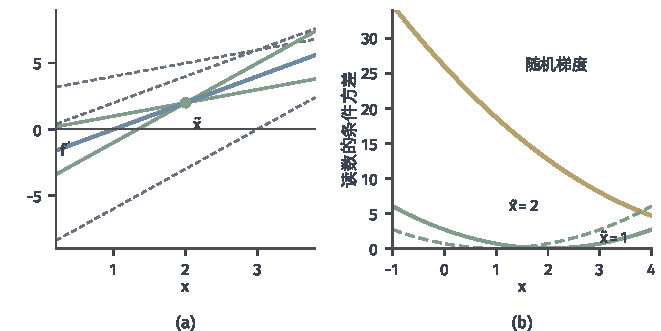
\includegraphics[width=112mm]{figures/05-optimization/05-stochastic-optimization/matplotlib/sgd-svrg-fan/figure.pdf}
  \caption{SVRG的纠偏，三项目标，快照$\tilde{x}=2$。(a)虚线是原始的三项读数，绿线是修正后的读数，蓝线是$f'$。修正后的三条线都经过快照处的点$(2,f'(2))$。(b)读数的条件方差随$x$的变化：黄线是普通随机梯度，绿实线是快照$\tilde{x}=2$，绿虚线是快照$\tilde{x}=1=x^\star$。}
  \label{fig:sgd-svrg-fan}
\end{BookInlineFigure}

图~\ref{fig:sgd-svrg-fan}(a)说明了修正的几何含义：原始的三条读数线各自散开，修正后都绕着快照处的完整梯度旋转，$x$越接近快照，分散越小。条件方差的表达式是$\tfrac23(x-\tilde{x})^2$，它在$x=\tilde{x}$处为零，这正是图(b)的绿线。比较$x=1$这一点，快照$\tilde{x}=2$时条件方差是$2/3$，普通随机梯度是$56/3$。

快照要不断更新。随着$\bm{x}$收敛，把快照移过来，图(b)的绿线就从实线变成虚线，方差在解处变成零。这样，算法每隔若干步要花一次完整梯度的成本重新设置快照，因此有内外两层循环，如图~\ref{fig:sgd-svrg-loop}所示。

\begin{BookInlineFigure}
  \centering
  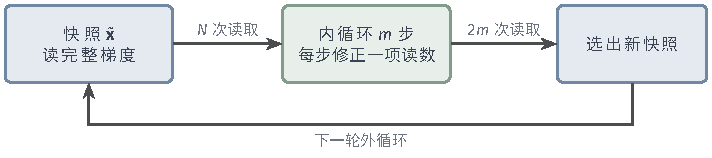
\includegraphics[width=110mm]{figures/05-optimization/05-stochastic-optimization/tikz/sgd-svrg-loop/figure.pdf}
  \caption{SVRG的两层循环。外循环计算完整梯度（$N$次读取）并存下快照，内循环运行$m$步，每步用式~\eqref{eq:sgd-svrg-direction}，读取同一项在两点的梯度（$2$次读取）。一轮外循环共$N+2m$次读取。}
  \label{fig:sgd-svrg-loop}
\end{BookInlineFigure}

\needspace{6\baselineskip}
\paragraph{变量}
\begin{itemize}
 \item $\tilde{\bm{x}}\in\mathbb{R}^n$：快照点。
 \item $\tilde{\bm{g}}\in\mathbb{R}^n$：快照点的完整梯度$\nabla f(\tilde{\bm{x}})$。
 \item $\bm{x}^{(t)}\in\mathbb{R}^n$：内循环的当前点，$t=0,\ldots,m$。
 \item $\alpha>0$，$m$：步长和内循环长度。
\end{itemize}

\paragraph{初始化}
取初始快照$\tilde{\bm{x}}$。例中取$\tilde{x}=2$，$\alpha=0.05$，这满足后面定理的条件，由式~\eqref{eq:sgd-example-gradients}，
\[
 \tilde{g}=f'(2)=2.
\]

\paragraph{每轮更新}
外循环的一轮按下列步骤进行。

\begin{enumerate}
 \item 快照：置$\bm{x}^{(0)}=\tilde{\bm{x}}$，计算$\tilde{\bm{g}}=\nabla f(\tilde{\bm{x}})$，共$N$次读取。例中$x^{(0)}=2$，$\tilde{g}=2$。
 \item 内循环：对$t=0,\ldots,m-1$，抽下标$i^{(t)}$，按式~\eqref{eq:sgd-svrg-direction}得到方向$\hat{\bm{g}}^{(t)}$，沿它走步长$\alpha$得到新点。

 例中第一步抽到$i=3$，$x^{(0)}=\tilde{x}$，方向就是完整梯度，
 \[
  \hat{g}^{(0)}=2,\qquad x^{(1)}=2-0.05\cdot2=1.9.
 \]

 第二步抽到$i=1$，$a_1=1$，方向和新点是
 \[
  \hat{g}^{(1)}=1\cdot(1.9-2)+2=1.9,\qquad x^{(2)}=1.9-0.05\cdot1.9=1.805.
 \]

 第三步抽到$i=2$，$a_2=2$，方向和新点是
 \[
  \hat{g}^{(2)}=2\cdot(1.805-2)+2=1.61,\qquad x^{(3)}=1.805-0.05\cdot1.61=1.7245.
 \]
 \item 选取新快照：从内循环的点中选一个作为新的$\tilde{\bm{x}}$。下面的定理要求在$\bm{x}^{(0)},\ldots,\bm{x}^{(m-1)}$中均匀随机选取，实践中也常取最后一点。
\end{enumerate}

外循环达到预定轮数后结束。最终得到最后一次的快照。例中三步都朝$x^\star=1$靠近，方向全部为正，没有再出现单项读数$-3$带来的上坡，这正是控制变量的效果。

\paragraph{差分的方差与收敛}
证明方差自动减小的关键，是用目标差控制逐项梯度的差。需要假设每一项都是光滑的凸函数。

\begin{lemma}[逐项梯度差的控制]
\label{lem:sgd-gradient-difference}
设$f_i$凸且梯度$L$-Lipschitz，$f=\frac1N\sum_if_i$有最小点$\bm{x}^\star$。则对任意$\bm{x}$，
\begin{equation}
 \frac{1}{N}\sum_{i=1}^{N}\lVert\nabla f_i(\bm{x})-\nabla f_i(\bm{x}^\star)\rVert_2^2\leq2L\bigl(f(\bm{x})-f^\star\bigr).
 \label{eq:sgd-gradient-difference}
\end{equation}
\end{lemma}

\begin{proof}
定义
\[
 \psi_i(\bm{x})=f_i(\bm{x})-f_i(\bm{x}^\star)-\langle\nabla f_i(\bm{x}^\star),\bm{x}-\bm{x}^\star\rangle.
\]
$\psi_i$凸，梯度$L$-Lipschitz，$\nabla\psi_i(\bm{x}^\star)=\bm{0}$，所以$\bm{x}^\star$是它的最小点，最小值为$0$。

对$\psi_i$从$\bm{x}$走一步$\bm{x}-\nabla\psi_i(\bm{x})/L$，由下降引理，
\[
 0\leq\psi_i\Bigl(\bm{x}-\frac{1}{L}\nabla\psi_i(\bm{x})\Bigr)\leq\psi_i(\bm{x})-\frac{1}{2L}\lVert\nabla\psi_i(\bm{x})\rVert_2^2.
\]

$\nabla\psi_i(\bm{x})$就是$\nabla f_i(\bm{x})$与$\nabla f_i(\bm{x}^\star)$的差。对$i$平均时，由$\nabla f(\bm{x}^\star)=\bm{0}$，一次项消失，$\psi_i$的平均恰为$f(\bm{x})-f^\star$。整理即得式~\eqref{eq:sgd-gradient-difference}。
\end{proof}

\begin{theorem}[SVRG的线性收缩]
\label{thm:sgd-svrg}
设每个$f_i$凸且梯度$L$-Lipschitz，$f$是$\mu$强凸的。设$0<\alpha<1/(4L)$，$m$足够大，使
\begin{equation}
 \rho=\frac{1}{\mu\alpha(1-2L\alpha)m}+\frac{2L\alpha}{1-2L\alpha}<1.
 \label{eq:sgd-svrg-rate}
\end{equation}
每轮外循环的新快照在$\bm{x}^{(0)},\ldots,\bm{x}^{(m-1)}$中均匀随机选取。则相邻两轮的快照$\tilde{\bm{x}}_{s}$，$\tilde{\bm{x}}_{s+1}$满足
\begin{equation}
 \mathbb{E}[f(\tilde{\bm{x}}_{s+1})]-f^\star\leq\rho\bigl(\mathbb{E}[f(\tilde{\bm{x}}_s)]-f^\star\bigr).
 \label{eq:sgd-svrg-contraction}
\end{equation}
\end{theorem}

\begin{proof}
固定一轮外循环，$\tilde{\bm{x}}$由此前的历史确定。记$\bm{x}=\bm{x}^{(t)}$，$E_x=f(\bm{x})-f^\star$，$E_s=f(\tilde{\bm{x}})-f^\star$。先控制方向的二阶矩。

在方向~\eqref{eq:sgd-svrg-direction}中加减$\nabla f_i(\bm{x}^\star)$，把它写成两段之和，再用不等式$(a+b)^2\leq2a^2+2b^2$，得到
\[
 \lVert\hat{\bm{g}}\rVert_2^2\leq2\lVert\nabla f_i(\bm{x})-\nabla f_i(\bm{x}^\star)\rVert_2^2+2\lVert\nabla f_i(\tilde{\bm{x}})-\nabla f_i(\bm{x}^\star)-\nabla f(\tilde{\bm{x}})\rVert_2^2.
\]

第二段里，$\nabla f_i(\tilde{\bm{x}})-\nabla f_i(\bm{x}^\star)$的条件均值恰为$\nabla f(\tilde{\bm{x}})$，第二段就是它减去自己的均值。方差不超过二阶矩，所以去掉$\nabla f(\tilde{\bm{x}})$后条件期望不会变小。对两段分别用式~\eqref{eq:sgd-gradient-difference}，得到
\[
 \mathbb{E}[\lVert\hat{\bm{g}}\rVert_2^2\mid\mathcal{F}^{(t)}]\leq4L(E_x+E_s).
\]

再展开距离。由条件无偏和$f$的凸性，内积项不小于$E_x$，于是
\[
 \mathbb{E}[\lVert\bm{x}^{(t+1)}-\bm{x}^\star\rVert_2^2\mid\mathcal{F}^{(t)}]\leq\lVert\bm{x}-\bm{x}^\star\rVert_2^2-2\alpha E_x+4L\alpha^2(E_x+E_s).
\]

对$t=0,\ldots,m-1$求和取全期望，距离项相消，并丢掉非负的终点距离。记$\bar{E}$为内循环点目标差的平均，它也是随机选出的新快照的期望目标差，得到
\[
 2\alpha(1-2L\alpha)m\bar{E}\leq\mathbb{E}\lVert\tilde{\bm{x}}-\bm{x}^\star\rVert_2^2+4L\alpha^2m\mathbb{E}[E_s].
\]

强凸性给出快照点的距离上界$\tfrac{2}{\mu}E_s$，代入后得到
\[
 2\alpha(1-2L\alpha)m\bar{E}\leq\Bigl(\frac{2}{\mu}+4L\alpha^2m\Bigr)\mathbb{E}[E_s].
\]
两边除以$2\alpha(1-2L\alpha)m$，即得式~\eqref{eq:sgd-svrg-contraction}。
\end{proof}

式~\eqref{eq:sgd-svrg-rate}的两项分别表示：内循环够长，初始距离的影响才能被摊薄；步长够小，快照带来的方差项才小于收缩。这里$L$是单项的光滑常数，在三项目标上$L=3$，$\mu=2$。取$\alpha=0.05<1/12$，$m=50$，得到
\[
 \rho=\frac{1}{2\cdot0.05\cdot0.7\cdot50}+\frac{0.3}{0.7}\approx0.286+0.429=0.714.
\]
这是一个保守的上界。三项目标从$\tilde{x}=2$开始一轮的实际结果，用$20000$次独立运行的平均来估计，目标差约从$1$降到$0.115$。

\paragraph{成本}
一轮外循环需要$N+2m$次读取，每轮把目标差减小一个固定比例。取$\alpha$为$1/L$的小常数倍、$m$与$\kappa$同量级时$\rho$是小于$1$的常数，所以减小一个固定比例约需$N+\kappa$量级的读取，这里$\kappa=L/\mu$用单项的光滑常数计算。完整梯度下降减小同样的比例约需$N\kappa_f$量级的读取，其中$\kappa_f$用$f$本身的光滑常数计算。$N$很大时前者优势明显。存储上，SVRG只保存$\tilde{\bm{x}}$和$\tilde{\bm{g}}$两个向量，每步重新计算$\nabla f_i(\tilde{\bm{x}})$。也可以事先保存所有项的快照梯度，每步只需一次读取，但内存要多$N$个向量。内循环长度$m$、快照的频率，在理论和实践之间常有差别，定理的$m$往往偏大。

SVRG要求能重复访问所有项，且每轮要算一次完整梯度，所以只适用于有限和目标；样本源源不断的期望目标不能直接用。

\subsection{SAGA}
\label{sec:sgd-saga}

SVRG要定期花一次完整梯度来设置快照。如果把每一项上次读到的梯度都记下来，是不是不用专门做快照，靠记忆逐步更新就够了？这就是SAGA\scite{defazio2014saga}的想法。

\paragraph{主要思想}
为每一项维护一个存下的旧梯度$\bm{\phi}_i$，以及它们的均值$\bar{\bm{\phi}}=\frac1N\sum_i\bm{\phi}_i$。每一步抽$i$，用新读数减去这一项的旧读数，再加上旧均值：
\begin{equation}
 \hat{\bm{g}}=\nabla f_i(\bm{x})-\bm{\phi}_i+\bar{\bm{\phi}}.
 \label{eq:sgd-saga-direction}
\end{equation}
这与SVRG的方向形式相同，只是把快照点的梯度换成了各项自己记录的旧梯度。给定历史，表项都是确定的，对$i$求条件平均，第二、三项相消，所以方向条件无偏。

完成参数更新之后，才把表项$\bm{\phi}_i$替换成新读数，并同步修改均值：
\begin{equation}
 \bar{\bm{\phi}}\leftarrow\bar{\bm{\phi}}+\frac{1}{N}\bigl(\nabla f_i(\bm{x})-\bm{\phi}_i\bigr).
 \label{eq:sgd-saga-mean}
\end{equation}
这个次序不能交换。若先把$\bm{\phi}_i$换成新读数，方向就变成$\bar{\bm{\phi}}$，只是旧梯度的平均，新读数根本没有进入更新，条件无偏也失去了。

\needspace{6\baselineskip}
\paragraph{变量}
\begin{itemize}
 \item $\bm{x}^{(t)}\in\mathbb{R}^n$：当前点。
 \item $\bm{\phi}_i\in\mathbb{R}^n$，$i=1,\ldots,N$：各项记录的旧梯度，共$N$个向量。
 \item $\bar{\bm{\phi}}\in\mathbb{R}^n$：表项的均值，用式~\eqref{eq:sgd-saga-mean}增量更新，不必每次重算。
 \item $\alpha>0$：步长。
\end{itemize}

\paragraph{初始化}
在初始点读全部$N$项填满梯度表，$N$次读取。例中取$x^{(0)}=2$，$\alpha=0.05$，表项和均值是
\[
 (\phi_1,\phi_2,\phi_3)=(5,4,-3),\qquad \bar{\phi}=2.
\]

\paragraph{每轮更新}
对$t=0,1,\ldots$依次执行以下步骤。

\begin{enumerate}
 \item 抽样并读取：抽$i^{(t)}$，计算新读数$\nabla f_{i^{(t)}}(\bm{x}^{(t)})$，这是一次读取。例中第一轮抽到$i=3$，新读数是$-3$。
 \item 计算方向并更新：由式~\eqref{eq:sgd-saga-direction}，例中第一轮
 \[
  \hat{g}^{(0)}=-3-(-3)+2=2,\qquad x^{(1)}=2-0.05\cdot2=1.9.
 \]
 \item 更新表项：把$\bm{\phi}_{i^{(t)}}$换成新读数，按式~\eqref{eq:sgd-saga-mean}修改均值。例中第一轮新读数与旧表项相同，$\phi_3$和均值都不变。
\end{enumerate}

例中第二轮抽到$i=1$，新读数$f_1'(1.9)=4.9$，方向和新点是
\[
 \hat{g}^{(1)}=4.9-5+2=1.9,\qquad x^{(2)}=1.9-0.05\cdot1.9=1.805.
\]
然后$\phi_1$变成$4.9$，均值变成$(4.9+4-3)/3\approx1.967$。

例中第三轮抽到$i=2$，新读数$f_2'(1.805)=3.61$，方向和新点是
\[
 \hat{g}^{(2)}\approx3.61-4+1.967=1.577,\qquad x^{(3)}\approx1.805-0.05\cdot1.577=1.726.
\]
然后$\phi_2$变成$3.61$，均值变成$(4.9+3.61-3)/3\approx1.837$。图~\ref{fig:sgd-saga-table}画出了表的变化。

\begin{BookInlineFigure}
  \centering
  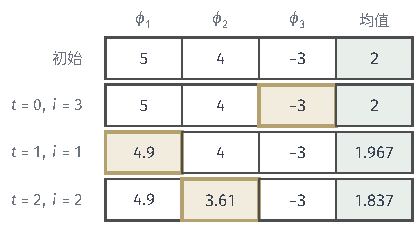
\includegraphics[width=72mm]{figures/05-optimization/05-stochastic-optimization/tikz/sgd-saga-table/figure.pdf}
  \caption{SAGA的梯度表在三步内的变化。每行是完成该步之后的表，黄框是刚被替换的项，右列是表的均值。第一步新读数恰好等于旧表项，表不变；此后只有被抽到的项发生变化。}
  \label{fig:sgd-saga-table}
\end{BookInlineFigure}

迭代在读取量达到预定预算后结束，最终得到$\bm{x}^{(T)}$；例中三步后$x^{(3)}\approx1.726$，每步一次读取，加上初始化的三次，共六次读取。

\paragraph{两种误差共同评价}
SAGA的状态比普通方法多一张表，所以进展要同时看两件事：参数离解多远，表项离各自的$\nabla f_i(\bm{x}^\star)$多远。参数接近解之后，表项还可能很旧，方差还不会小。要让方差趋于零，就需要每一项都被更新到解附近。

\begin{theorem}[SAGA的线性收敛]
\label{thm:sgd-saga}
设每个$f_i$凸且梯度$L$-Lipschitz，$f$是$\mu$强凸的，取$\alpha=1/(3L)$，下标独立均匀抽取，梯度表在初始点填满。则存在只依赖初始距离和初始表项误差的常数$C$，使
\begin{equation}
 \mathbb{E}[\lVert\bm{x}^{(T)}-\bm{x}^\star\rVert_2^2]\leq\Bigl(1-\min\Bigl\{\frac{1}{4N},\frac{\mu}{3L}\Bigr\}\Bigr)^TC.
 \label{eq:sgd-saga-rate}
\end{equation}
\end{theorem}

式~\eqref{eq:sgd-saga-rate}的证明需要构造一个同时包含距离和各表项误差的函数，并证明它的期望按上述比例收缩，推导较长，读者可查阅原始论文\scite{defazio2014saga}。这里解释结论的机制。速率的最小值中有两项：$\mu/(3L)$与单纯的梯度下降类似，由条件数决定；$1/(4N)$反映表项的刷新速度，每一步只刷新一项，刷新一遍大约需要$N$步。$N$很大时，记忆更新是瓶颈，反过来则是条件数决定收敛。

在三项目标上，$N=3$，$L=3$，$\mu=2$，所以
\[
 \min\Bigl\{\frac{1}{12},\frac29\Bigr\}=\frac{1}{12},
\]
定理保证的是每步收缩$11/12$。手算所用的$\alpha=0.05$小于$1/(3L)=1/9$，只用来演示表项的变化。

SAGA没有强凸性时也有保证，平均点的目标差按$1/T$的量级下降，常数与$N$有关，这里不再讨论。

\paragraph{比较}
表~\ref{tab:sgd-vr-compare}按读取和存储比较这些方法。方差控制的共同代价是：多读或多存，并依赖逐项光滑、凸性等结构。

\begin{BookInlineTable}
  \centering
  \begin{tabular}{llll}
    \toprule
    方法 & 每次更新读取 & 存储 & 需要重复访问\\
    \midrule
    随机梯度 & $1$ & $1$个向量 & 否\\
    小批量 & $B$ & $1$个向量 & 否\\
    SVRG & $2$，另有每轮$N$ & $2$个向量 & 是\\
    SAGA & $1$，初始化$N$ & $N+2$个向量 & 是\\
    \bottomrule
  \end{tabular}
  \caption{方差控制方法的成本。存储只计迭代所需向量，随机梯度和小批量含当前点。}
  \label{tab:sgd-vr-compare}
\end{BookInlineTable}

SAGA的表要存$N$个$n$维向量，这在$N$和$n$都很大时是沉重的负担。对各项梯度是某个数乘已知向量的线性模型，每个表项只需存一个标量，才算切实可行。

图~\ref{fig:sgd-vr-cost}用一个$N=500$、$n=20$的正则最小二乘实例比较总读取量。横轴是读取量除以$N$，即完整遍历的轮数。随机梯度初期最快，但很快到达噪声底。完整梯度稳定下降，但每步代价是$N$。SVRG和SAGA在初期略慢于随机梯度，此后保持线性收敛，目标差继续下降到比噪声底小许多个量级的水平。

\begin{BookInlineFigure}
  \centering
  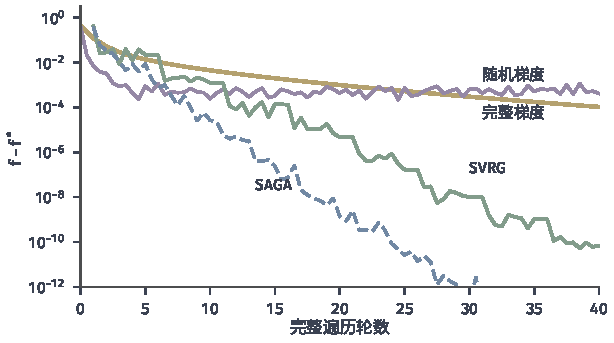
\includegraphics[width=104mm]{figures/05-optimization/05-stochastic-optimization/matplotlib/sgd-vr-cost/figure.pdf}
  \caption{总读取量与目标差，$N=500$、$n=20$的正则最小二乘实例（种子固定），$\lVert\bm{a}_i\rVert_2=1$，$\gamma=0.005$。黄线是完整梯度，紫线是固定步长$0.1$的随机梯度，绿线是SVRG（$\alpha=0.2/L$，$m=2N$，此处$L$取单项的光滑常数），蓝色虚线是SAGA（$\alpha=1/(3L)$）。横轴是读取量除以$N$，纵轴取对数。}
  \label{fig:sgd-vr-cost}
\end{BookInlineFigure}

这个比较的结论有边界：只针对这一个实例和这一组参数，SVRG和SAGA的优势在需要高精度时才明显。若只需低精度，或者问题本身的噪声底已经够用，普通随机梯度加小批量更简单；若数据是流式的，不能重复访问，这两种方法都用不上。
